%%%%%%%%%%%%%%%%%%%%%%%%%%%%%%%%%%%%%%%%%%%%%%%%%%%%%%%%%%%%%%%%%%%%%%%%
% This is the introduction chapter file.
%%%%%%%%%%%%%%%%%%%%%%%%%%%%%%%%%%%%%%%%%%%%%%%%%%%%%%%%%%%%%%%%%%%%%%%%
%
% Author:   René Widmer
%           Institute for Surgical Technology and Biomechanics ISTB
%           University of Bern
%           rene.widmer@istb.unibe.ch
%
% Date:     10/28/2009
%
%%%%%%%%%%%%%%%%%%%%%%%%%%%%%%%%%%%%%%%%%%%%%%%%%%%%%%%%%%%%%%%%%%%%%%%%

\chapter{Introduction}

\textit{The introduction provides a thorough review of the background, including relevant literature, the motivation, the aims of the thesis and the hypotheses. Literature references for the thesis should be collected in one common bibliography at the end of the thesis.}

\vskip1em

With the population aging, medicine is recognizing the major impact of osteoporosis on health and function. The chief manifestation of osteoporosis is the pathologic fracture. Osteoporotic patients sustain fractures when minimal force is applied to weakened, discontinuous bone. Traditionally, most attention has been given to osteoporotic fractures of the hip. However, the 700'000 osteoporotic vertebral compression fractures per year in the United States easily outnumber fractures of the hip and ankle combined.

It is estimated that more than 200 million people worldwide are currently affected by osteoporosis, and 100 million are at risk of suffering from related complications. It is a proven fact that solely in Europe about 3.8 million osteoporotic fractures were treated in the year 2000. The prevalence of the disease is expected to rise significantly with the aging population: In the US, the number of annual osteoporosis-attributable fractures is expected to double by the year 2025, and the growth predictions for Switzerland are of comparable magnitude. The total cost of osteoporotic fractures in the US was estimated at 7 - 10 billion dollars in 1995 for a population of 250 million, and expenditures for the treatment of vertebral fractures alone were estimated at 377 million Euros in 2003 in the European Union.

Vertebral compression fractures have previously received limited attention from the spine care community. This oversight may be a result of the perception that vertebral compression fractures are benign, self-limited problems or that treatment options are limited. However, it has become clear that vertebral compression fractures are associated with significant physiologic and functional impairment, even in patients not presenting for medical evaluation at the time of fracture.

Open surgery is fraught with morbidity and implant failure in this frail patient population. Therefore, nonoperative management, including medications and bracing, has been recommended for the vast majority of patients. Unfortunately, large numbers of patients report intractable pain and inability to return to activities. The limitations of nonoperative management have encouraged increasing interest in new, percutaneous methods of fracture stabilization that allow early return to activity and do not require fixation in weak bone.

Percutaneous vertebroplasty was first performed in France in the mid 1980s, and there is extensive experience with the technique in continental Europe. Originally used to treat the painful, aggressive variant of vertebral haemangioma\footnote{A haemangioma describes a benign overgrowth of blood vessels.}, percutaneous vertebroplasty has been applied to painful vertebral lesions caused by metastatic disease and painful osteoporotic fractures.

Osteoporosis is a skeletal disorder which is characterized by loss of bone mass and degradation of trabecular structure, which results in an increased fracture risk. Osteoporotic fractures most frequently occur in structures subjected to large strains, such as the spine or the hip, or bones commonly affected by falls, such as the distal forearm. Thoracic and lumbar vertebral collapses are recognized as the most frequent complication resulting from the loss of bony substance.

\vskip1em
\noindent\textit{etc.}

\begin{figure}[htbp]
	\centering
	\subfloat[Normal]
	{
		\label{fig:subfig:NormalStructure}
		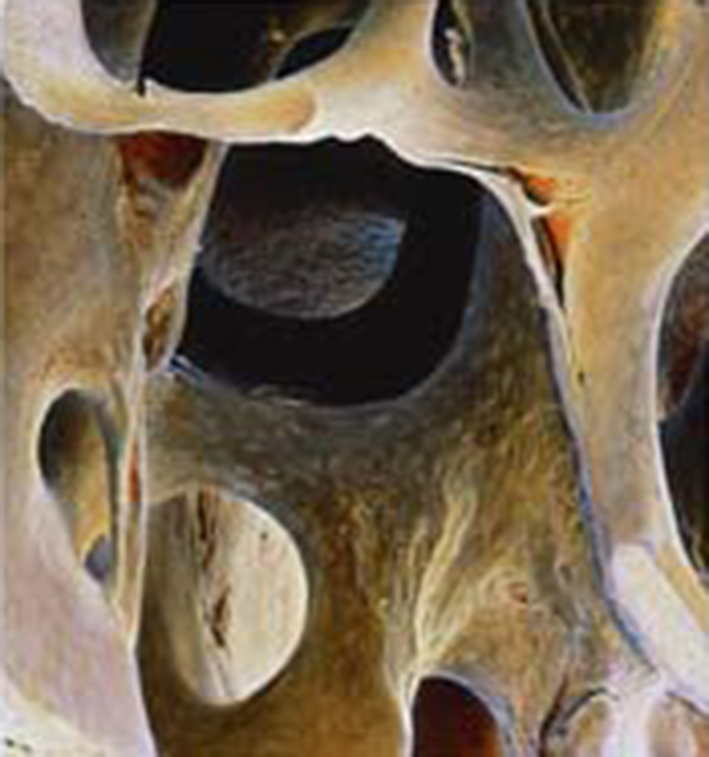
\includegraphics[width=4.5cm]{NormalBoneStructure}
	}
	\hfill
	\subfloat[Osteoporotic]
	{
		\label{fig:subfig:OsteoporoticStructure}
		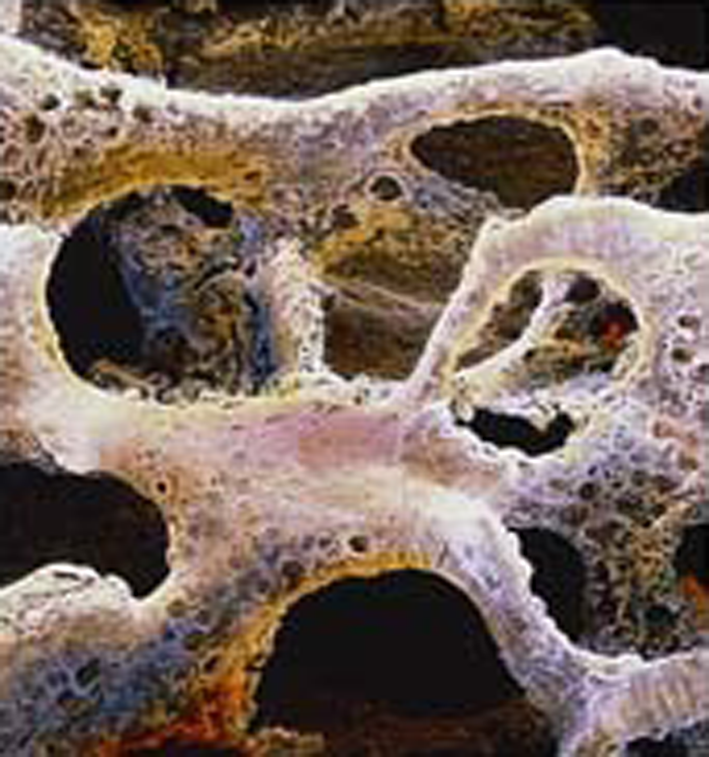
\includegraphics[width=4.5cm]{OsteoporoticBoneStructure}
	}
	\caption[Normal and osteoporotic spongy bone structure]{Normal and osteoporotic spongy microscale bone structure at 25x magnification. Image source: \url{http://facstaff.unca.edu/cnicolay/BIO223-F08/L06-bone.pdf}.\par\vspace{1em}\textit{Please document your image sources.}}
	\label{fig:OsteoporoticStructure}  
\end{figure}


\endinput